\chapter{2012} 
\section*{一、单项选择题(本大题共 20 小题,每小题 2 分,共 40 分)}

1. (   )是数据的最小单位。

A. 数据元素 B. 数据项 C. 数据对象 D. 数据结构

2. 在长度为 \(\mathrm{n}\) 顺序实现的线性表的第 \(\mathrm{i}\left( {1 \leq  \mathrm{i} \leq  \mathrm{n}}\right)\) 个位置删除一个元素,需要前移(   )个元素。

A. n-i+1 B. i C. 1 D. n-i

3. 单链表的存储密度(   )。

A. 大于 1 B. 等于 1 C. 小于 1 D. 不能确定

4. 将长度为 \(\mathrm{n}\) 的单链表链接在长度为 \(\mathrm{m}\) 的单链表之后的算法的时间复杂度为 (   )。

A. \(\mathrm{O}\left( 1\right)\) B. \(\mathrm{O}\left( \mathrm{n}\right)\) C. \(\mathrm{O}\left( \mathrm{m}\right)\) D. \(O\left( {m + n}\right)\)

5. 设计一个把十进制数转换为八进制数的算法, 采用 (   ) 数据结构最佳。

A. 栈 B. 队列 C. 顺序结构线性表 D. 链式结构线性表

6. 一个栈的输入序列为 a, b, c, d, 下面哪一个序列不可能是这个栈的输出序列？(   )

A. b, c, d, a B. d, c, a, b

C. a. c. b. d D. c, d, b, a

7. 若用一个大小为 6 的数组来实现循环队列, 且当前 rear 和 front 的值分别为 0 . 和 3。当从队列删除两个元素,再加入一个元素后, rear 和 front 的值分别为 (   ).

A. 1 和 5 B. 2 和 4 C. 4 和 2 D. 5 和 1

8. 若串 S = "database",其非空子串数目为(   )。

A. 8 B. 37 C. 36 D. 9

9. 数组 a 中,每个元素 a[i, j]的长度为 4 个字节,行下标 i 从 0 到 7 ,列下标 j 从 0 到 9 ,从首地址连续存放在存储器内,该数组按行优先存放时,元素 a[7][4] 的起始地址为(   )。

A. a + 192 B. a +188 C. a +300 D. a +296

10. 若广义表 L 满足 Head(L) = Tail(L), 则 L 为 (   )。

A. (   ) B. \(\left( \left( \;\right) \right)\) C. \(\left( {\left( \right) ,\left( \right) }\right)\)  \(D.\left( {\left( ,\right) ,\left( \;\right) ,\left( \;\right) }\right)\)

11. 设高度为 \(\mathrm{h}\) 的二叉树上只有度为 0 和度为 2 的结点,则此二叉树中至少有 (   )个结点。

A. \(2\mathrm{\;h}\) B. \(2\mathrm{\;h} - 1\) C. \(2\mathrm{h} + 1\) D. \(h + 1\)

12. 对二叉树所有结点进行编号(从 1 开始),要求每个结点的编号大于其左右孩 子的编号,同一结点的左右孩子中,其左孩子的编号小于其右孩子的编号, 则可采用(   )次序的遍历实现编号。

A. 先序 B. 中序 C. 后序 D. 从根开始的层次遍历

13. G 是一个连通图,共有 28 条边,则该图至少有(   )个顶点。

A. 6 B. 7 C. 8 D. 9

14. 若一个具有 \(\mathrm{n}\) 个顶点, \(\mathrm{k}\) 条边的无向图是一个森林 \(\left( {\mathrm{N} > \mathrm{K}}\right)\) ,则该森林中必有 (   )颗树。

A. 1 B. \(\mathrm{k}\) C. n D. n-k

15. 在二叉排序树中,关键值最大的结点(   )。

A. 左指针一定为空 B. 右指针一定为空

C. 左右指针均为空 D. 左右指针均不为空

16. 含有 12 个结点的平衡二叉树的最大深度是(   )。

A. 3 B. 4 C. 5 D. 6

17. 在非空 m 阶 B-树上,除根结点以外的所有其他非终端结点(   )。

A. 至少含有 \(\lceil m/2\rceil\) 棵子树 B. 至多含有 \(\lceil \mathrm{m}/2\rceil\) 棵子树

C. 至少含有 \(\lfloor m/2\rfloor\) 棵子树 D. 至多含有 \(\lfloor m/2\rfloor\) 棵子树

18. 下列序列中. (   )是执行第一趟快速排序后得到的序列(排序的关键字类型是字符串)。

A. [da, ax, eb, de, bb] fp [hq, gv]

B. \(\left\lbrack  {{cd},{eb},{ax},{da}}\right\rbrack  {fp}\left\lbrack  {{hq},{gv},{bb}}\right\rbrack\)

C. \(\left\lbrack  {{gv},{ax},{eb},{cd},{bb}}\right\rbrack  {fp}\left\lbrack  {{da},{hq}}\right\rbrack\) 

D. [ax, bb, cd.da] fp [eb, gv, hq]

19. 在文件“局部有序”的情况下,最佳内部排序是(   )。

A. 直接插入排序 B. 快速排序 C. 简单选择排序 D. 归并排序

20. 时间复杂度不受待排序序列初始状态的影响,总是 \(\mathrm{O}\left( {\mathrm{n}}^{2}\right)\) 的是(   )。

A. 直接插入排序 B. 快速排序 C. 简单选择排序 D. 归并排序

\section*{二、填空题(本大题共16小题,每小题2分,共32分)}

1. 若一个算法的语句频度之和是 T(n) = 15n+10nlogn,则算法的时间复杂度为\_\_\_\_\_。  

2. 表长为n的线性表,当在任何位置上插入或删除一个元素的概率相等时,插入一个元素需移动元素的平均个数为\_\_\_\_\_。  

3. 设栈S和队列Q的初始状态皆为空,元素a、b、c、d、e和f依次通过一个栈,一个元素出栈后即进入队列 \(\mathrm{Q}\) ,若6个元素出队列的顺序是 \(\mathrm{c}\text{ 、 }\mathrm{e}\text{ 、 }\mathrm{\;d}\text{ 、 }\mathrm{f}\) 、 b、a 则栈 S 至少应该容纳\_\_\_\_\_个元素。

4. 用数组 Q(其下标在 0...n-1,共有 n 个元素)表示一个循环队列, \(\mathrm{f}\) 为当前对头元素的前一位置, \(\mathrm{r}\) 为队尾元素位置,假定队列中元素个数总小于 \(\mathrm{n}\) ,求队列中元素个数的公式是\_\_\_\_\_。

5. 采用特殊字符作为串的结束,串 \(S =\) "Windows"需要至少长度为\_\_\_\_\_的字符数组存放。

6. 已知数组 \(\mathrm{A}\left\lbrack  {{1...10},{1...10}}\right\rbrack\) 为对称矩阵,其中每个元素占 4 个单元。现将其下三角部分按行优先次序存储在起始地址为 1000 的连续内存单元中,则元素 \(\mathrm{A}\lbrack 5\) , 6]对应的地址为\_\_\_\_\_。

7. 将一个 \(A\left\lbrack  {{0...99},{0...99}}\right\rbrack\) 的三对角矩阵,按行优先存入一维数组 \(B\left\lbrack  {0.297}\right\rbrack\) 中, \(A\) 中元素 \(\mathrm{A}\left\lbrack  {65}\right\rbrack  \left\lbrack  {65}\right\rbrack\) 在 \(\mathrm{B}\) 中的位置 \(\mathrm{k}\) 为\_\_\_\_\_。

8. 有 \(\mathrm{n}\) 个结点的二叉树,已知叶子结点个数为 \({\mathrm{n}}_{0}\) ,则度为 1 的结点的个数 \({\mathrm{n}}_{1}\) =\_\_\_\_\_。

9. 一棵有 124 个叶子结点的完全二叉树,最多有\_\_\_\_\_个结点。

10. 具有 n 个结点的满二叉树,其叶子结点有\_\_\_\_\_个。

11. 在序列(3,6,10,12,15,18,22,24,27,42,50)中采用折半查找(二分查找)方法查找元素 50,需要进行\_\_\_\_\_次元素之间的比较。

12. 有 n 个顶点的连通图用邻接矩阵表示时,该矩阵至少有\_\_\_\_\_个非零元素。

13. 下图的拓扑排序序列是\_\_\_\_\_。

\begin{center}
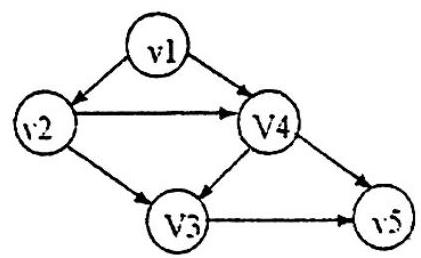
\includegraphics[width=0.3\textwidth]{images/2012/blanks_3.jpg}
\end{center}
\hspace*{3em} 

14. 若对序列(45,38,65,97,76,12,28,56)采用直接选择排序法排序,则第二趟结束后序列的状态是\_\_\_\_\_。

15. 高度为 4 的二叉平衡树最少有\_\_\_\_\_个结点。

16. 对于键值序列 \(\{ {11},{13},{10},{18},{50},{15},7,{20},{25},{90}\}\) ,建立初始堆,必须从键值为\_\_\_\_\_的结点开始对每个结点进行一次堆调整。

\section*{三、问答题(本大题共 6 小题,每小题 8 分,共 48 分)}

1. 在双循环链表中,写出在指针 \(\mathrm{p}\) 所指结点之后插入指针 \(\mathrm{s}\) 所指结点的执行语句序列。结点定义如下:

struct Node\{

\hspace*{1em} char data;

\hspace*{1em} Node *next;

\hspace*{1em} Node *prior;

\};

\vspace{5em}

2. 已知二叉树的先序序列和中序序列分别为 ABDGCEFH 和 DGBAECHF:

(1) 画出该二叉树;

(2)写出此二叉树的后序序列；

(3)画出与此二叉树对应的森林。
\vspace{5em}


\newpage
3. 已知由 12 个关键字构成的序列18、31、13、11、20、35、25、8、4、24、 40、27:

(1)请画出该序列的二叉排序树；

(2)给出删除结点 18 后的二叉排序树。
\vspace{5em}


4. 已知初始序列(50,80,63,45,48,92),写出直接插入排序的各趟排序的结果。
\vspace{5em}


\newpage
5. 设 Hash 函数为 \(\mathrm{H}\left( \mathrm{K}\right) = \mathrm{K}{\;\operatorname{mod}\;7}\) ,哈希表的地址空间为0,1,2,3,4,5,6, 开始时哈希表为空, 用二次探测再散列法解决冲突, 请画出依次插入键值 16 、 21、23、6、30、12、18 后的哈希表。
\vspace{8em}

6. 已知序列 45、15、20、35、25、60,请画出依次插入该序列的 AVL 树(平衡二叉树)。
\vspace{10em}

\section*{四、算法应用、分析题(本大题共 2 小题,第 1 小题 12 分,第 2 小题 8 分,共 20 分)}

1. 设一个无向网 \(G\) 如下:

\begin{center}
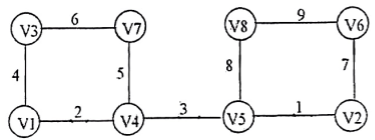
\includegraphics[width=0.6\textwidth]{images/2012/algorithm_1.png}
\end{center}


(1)请写出图 \(G\) 的邻接矩阵 \(A\) ；

(2)如果对某个顶点的邻接点的访问顺序按序号从小到大排列,请写出从顶点 \(\mathrm{v}1\) 出发,按“深度优先”和“广度优先”搜索方法遍历网 G 所得到的顶点序列: 

(3)从顶点 vl 出发,按照最小生成树的 Prim 算法,画出网 \(G\) 的一棵最小生成树。
\vspace{20em}

2. 已知某字符串 \(S\) 中共有 \(A\) 、 \(B\) 、 \(C\) 、 \(D\) 、 \(E\) 、 \(F\) 、 \(G\) 和 \(H\) 共 8 种字符,各种字符分别出现 2 次、1 次、4 次、5 次、7 次、3 次、4 次和 10 次,对该字符串用 \(\{ 0,1\}\) 进行前缀编码: 

(1)请画出对应的 Huffman 树,并给出各字符的前缀编码: 

(2)该字符串 \(S\) 的编码有多少位？
\vspace{20em}

\section*{五、算法设计题(本大题共 1 小题, 共 10 分)}

1. 有一个单链表 L (至少有一个结点),其头结点指针为 L,编写一个过程将 L 置逆,要求逆转在原链表上进行。单链表中的结点定义如下:

struct Node \{

\hspace*{1em} char data;

\hspace*{1em} Node *next;

\};
